\documentclass[12pt,a4paper]{article}%
\usepackage{amsmath}
\usepackage{amsfonts}
\usepackage{amssymb}
\usepackage{setspace}
\usepackage{listings}
\usepackage{graphicx}
\usepackage[normalem]{ulem}
\usepackage[T2A]{fontenc}
\usepackage[utf8]{inputenc}
\usepackage[english,russian]{babel}
%-------------------------------------------
\setlength{\textwidth}{7.0in}
\setlength{\oddsidemargin}{-0.35in}
\setlength{\topmargin}{-0.5in}
\setlength{\textheight}{9.0in}
\setlength{\parindent}{0.3in}
\graphicspath{{../plots/}}

\onehalfspacing


\begin{document}

\begin{titlepage}
  \begin{center}
    МИНОБРНАУКИ РОССИИ\\
    САНКТ-ПЕТЕРБУРГСКИЙ ГОСУДАРСТВЕННЫЙ\\
    ЭЛЕКТРОТЕХНИЧЕСКИЙ УНИВЕРСИТЕТ\\
    "ЛЭТИ" ИМ. В. И. ЛЕНИНА (УЛЬЯНОВА)\\
    Кафедра МО ЭВМ

    \vspace{4cm}

    ОТЧЕТ\\
    к практическому заданию №1
    \vfill

    \begin{tabular}{ c c c }
      Студент гр. 8303 & \uline{\hspace{3cm}} & Гришин К. И. \\[1cm]
      Преподаватель    & \uline{\hspace{3cm}} & Попова Е. В. \\
    \end{tabular}
    
    \vfill
    Санкт-Петербург\\
    2022
  \end{center}
\end{titlepage}


\section{Цель работы}
Найти решение задач матричных игр с нулевой суммой

\section{Задание}
Вариант 3

$$
\begin{aligned}
  C_1 &= &&
  \begin{pmatrix}
    2 & 2 & 6 & 5 \\
    3 & 3 & 7 & 7 \\
    4 & 3 & 4 & 2 \\
    5 & 6 & 2 & 4
  \end{pmatrix} \\ \vspace{0.5cm}\\
  C_2 &= &&
  \begin{pmatrix}
    2 & 7 \\
    4 & 3 
  \end{pmatrix} \\ \vspace{0.5cm}\\
  C_3 &= &&
  \begin{pmatrix}
    3 & 6 & 1 & 4 & 2 \\
    5 & 2 & 4 & 2 & 7
  \end{pmatrix} \\ \vspace{0.5cm}\\
  C_4 &= &&
  \begin{pmatrix}
    4 & 8 \\
    3 & 4 \\
    6 & 5 \\
    7 & 2 \\
    6 & 3 
  \end{pmatrix} \\ \vspace{0.5cm}\\
  C_5 &= &&
  \begin{pmatrix}
    2 & 1 & 3 \\
    5 & 2 & 4 \\
    3 & 7 & 5 
  \end{pmatrix} \\ \vspace{0.5cm}\\
\end{aligned}
$$

\pagebreak

\section{Ход выполнения работы}

\subsection{Определеить границы выигрыша и наличие седловой точки С1}
Для поиска седловых точек матричной игры использовалось инструментально средство:
\begin{lstlisting}[language=Python]
  import numpy as np

  def matrix_limits(matrix):
    return (
        max(np.apply_along_axis(lambda x: min(x), axis=1, arr=matrix)),
        min(np.apply_along_axis(lambda x: max(x), axis=0, arr=matrix))
    )
\end{lstlisting}

Получены следующие границы игры: (3, 5). Седловой точки нет.

\subsection{Графически и аналитически решить матричную игру 2x2 для матрицы C2}
Графически найдены вероятности для стратегий первого игрока:
\begin{center}
  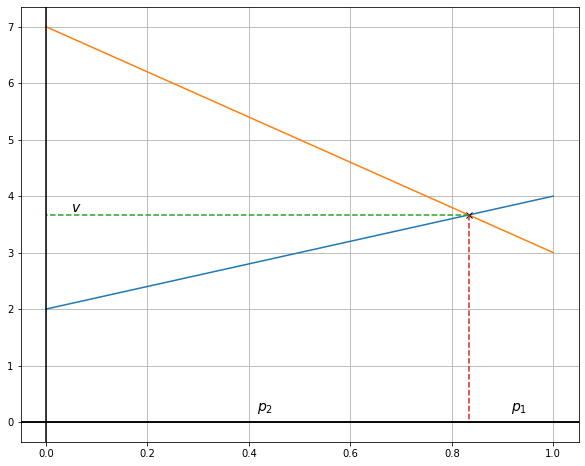
\includegraphics[scale=0.5]{C2.png}
\end{center}
$p_1 = 0.18$\\$p_2 = 0.82$\\$v = 3.7$

Аналитически найдены полученные значения:
$$
\begin{aligned}
  p_1 &= && \frac{3 - 4}                {2 + 3 - (7 + 4)} && = 0.17  \pm 0.08  \\ \vspace{0.5cm}\\
  p_2 &= && \frac{2 - 7}                {2 + 3 - (7 + 4)} && = 0.833 \pm 0.016 \\ \vspace{0.5cm}\\
  V   &= && \frac{2 \cdot 3 - 7 \cdot 4}{2 + 3 - (7 + 4)} && = 3.667 \pm 0.009
\end{aligned}
$$

\subsection{Графически и аналитически решить матричную игру 2xN для матрицы C3}
Графически найдены вероятности для стратегий первого игрока:
\begin{center}
  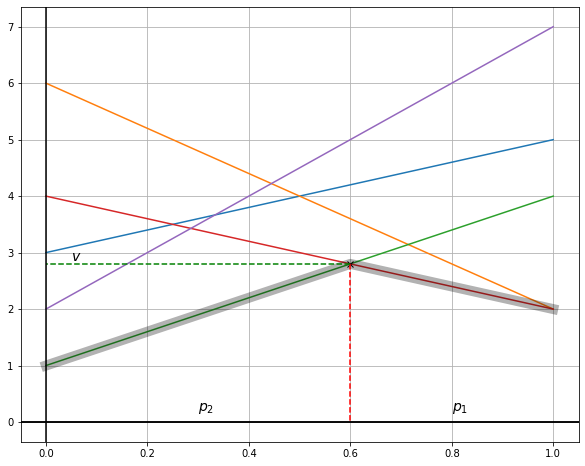
\includegraphics[scale=0.5]{C3.png}
\end{center}
$p_1 = 0.4$\\$p_2 = 0.6$\\$v = 2.8$

Аналитически найдены полученные значения:
$$
\begin{aligned}
  p_1 &= && \frac{4 - 2}                {4 + 4 - (1 + 2)} && = 0.4\\ \vspace{0.5cm}\\
  p_2 &= && \frac{4 - 1}                {4 + 4 - (1 + 2)} && = 0.6\\ \vspace{0.5cm}\\
  V   &= && \frac{4 \cdot 4 - 1 \cdot 2}{4 + 4 - (1 + 2)} && = 2.8
\end{aligned}
$$

\subsection{Графически и аналитически решить матричную игру Nx2 для матрицы C4}
Графически найдены вероятности для стратегий первого игрока:
\begin{center}
  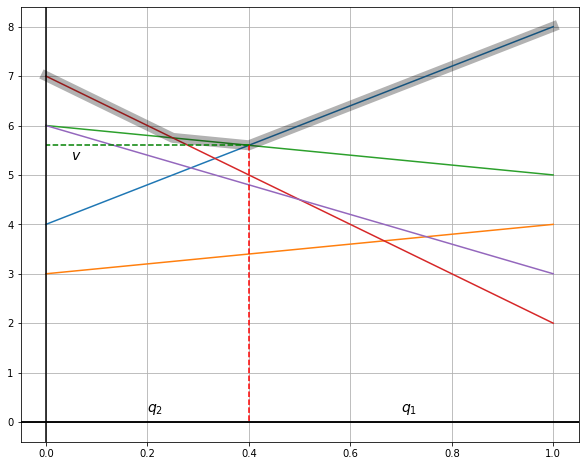
\includegraphics[scale=0.5]{C4.png}
\end{center}
$q_1 = 0.6$\\$q_2 = 0.4$\\$v = 5.6$

Аналитически найдены полученные значения:
$$
\begin{aligned}
  q_1 &= && \frac{8 - 5}                {6 + 8 - (5 + 4)} && = 0.6 \\ \vspace{0.5cm}\\
  q_2 &= && \frac{6 - 4}                {6 + 8 - (5 + 4)} && = 0.4 \\ \vspace{0.5cm}\\
  V   &= && \frac{8 \cdot 6 - 5 \cdot 4}{6 + 8 - (5 + 4)} && = 5.6
\end{aligned}
$$

\subsection{С помощью симплекс-метода решить матричную игру MxN для матрицы C5}
Границы значения игры: (3, 5)

Наибольший проигрыш второго игрока не может быть меньше $V$.
Следовательно матрицу С5 можно представить в виде системы
уравнений в смешанных стратегиях.
$$
\begin{aligned}
  2p_1+5p_2+3p_3 &\geq& V \\
  1p_1+2p_2+7p_3 &\geq& V \\
  3p_1+4p_2+5p_3 &\geq& V \\
  1p_1+1p_2+1p_3 &=& 1  
\end{aligned}
$$
Проведя замены $x = p / V$ и $Z = 1 / V$ получаем
$$
\begin{aligned}
  2x_1+5x_2+3x_3 &\geq& 1 \\
  1x_1+2x_2+7x_3 &\geq& 1 \\
  3x_1+4x_2+5x_3 &\geq& 1 \\
  1x_1+1x_2+1x_3 &=& Z
\end{aligned}
$$
То есть необходимо решить задачу линейного программирования
по минимизации функции $1x_1+1x_2+1x_3 = Z$.

\pagebreak
Для решения задачи линейного программирования использовался модуль SciPy.
\begin{lstlisting}[language=Python]
  from scipy.optimize import linprog
  def solve_matrix(matrix):
    objective_funciton_coefs = np.array([1, 1, 1])
    constraint_matrix = matrix.T * -1
    constraint_vector = np.array([-1, -1, -1])
    return linprog(
      objective_funciton_coefs,
      A_ub=constraint_matrix,
      b_ub=constraint_vector
    )
\end{lstlisting}
Значение $Z$: $0.2413793105018628$\\
Значения $x$: $[0.000000, 0.137931, 0.103448]$

\vspace{\baselineskip}
Проведем обратные преобразования для получения $p$ и $V$\\
Значение $V$: 4.143\\
Значения $p$: [0.000, 0.571, 0.429]

\end{document}